\chapter{Android jako system operacyjny}

\section{Początki systemu}
Słowo \textit{android} w czasach obecnych używane jest w wielu kontekstach. Może odnosić się ciągle do humanoidalnego robota, znanego nam z literatury science-fiction, ale ostatnio częściej kojarzone jest z rynkiem nowoczesnych telefonów komórkowych (tzw. smartfonów), tabletów i innych urządzeń przenośnych. Android to również nazwa firmy, system operacyjny, projekty open-source, a nawet społeczność programistów.

Początki systemu Android sięgają roku 2003, kiedy to Andy Rubin, Chris White, Nick Sears oraz Rich Miner założyli w Kaliforni firmę Android Inc. Głównym celem powstania firmy była chęć tworzenia urządzeń mobilnych, które bazowałyby na danych lokalizacyjnych i uwzględniały preferencje użytkowników. Jednak zmagająca się z wymaganiami rynku oraz trudnościami finansowymi firma w 2005 roku została przejęta przez Google Inc., amerykańskie przedsiębiorstwo z branży internetowej, słynące z popularnej wyszukiwarki o tej samej nazwie. Wkrótce potem założono grupę \textit{Open Handset Alliance} (OHA), w której skład weszły (oprócz Google) takie znane firmy jak HTC, Intel, Motorola, Qualcomm, T-Mobile, Sprint Nextel oraz NVIDIA, a która stawiała sobie za cel rozwój otwartych standardów dla telefonii mobilnej. Zdecydowanie przyspieszyło to badania nad systemem i jego rozwój. Pierwsza wersja Androida została przedstawiona światu już w 2007 roku, a pierwszym telefonem, który korzystał z tego systemu, był HTC G1.

Dwie premierowe wersje systemu nie miały nazw nadanych zgodnych z konwencją, do której przywykli użytkownicy z całego świata, ale począwszy od wersji 1.5, która została wydana 30 kwietnia 2009 roku, oficjalne wersje systemu otrzymywały już nazwy słodkich deserów lub smakołyków, zgodnie z porządkiem alfabetycznym. Wersja 1.5 otrzymała nazwę \textit{Cupcake}.

\section{Udział w rynku}
Android, jako system operacyjny przeznaczony dla urządzeń mobilnych, według portalu AntyWeb.pl w maju 2015 roku miał największy udział w rynku tych urządzeń w Polsce, a jego wartość w 2014 roku przekroczyłą 65 \%. 

\begin{figure}[!htb]
    \centering
    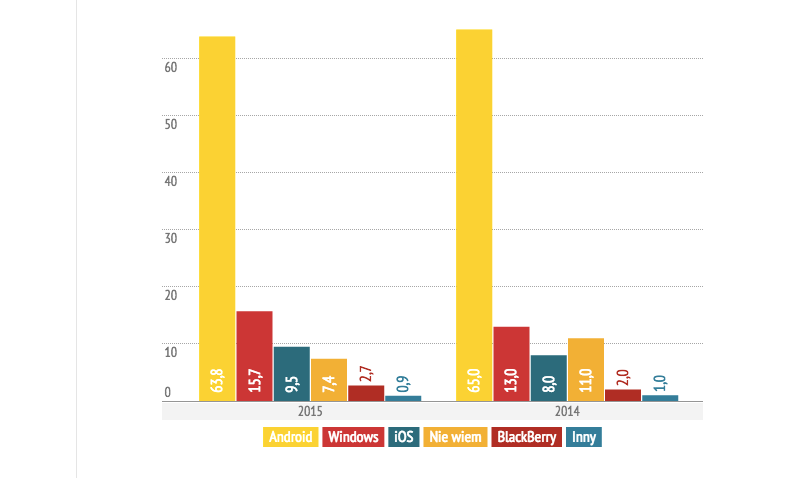
\includegraphics[width=15cm]{imgs/ch2_android_udzial_1.png}
    \caption
{Android – udział w rynku urządzeń mobilnych w Polsce. (Źródło: portal AntyWeb.pl, 05/2015)}
    \label{fig:android_udzial_polska}
\end{figure} 

Drugie miejsce, według tego samego portalu, zajmuje system Windows, a trzecie iOS. Na świecie proporcje udziału są nieco inne, ale ciągle na czele jest system Android, z wynikiem ponad 53\%. Na drugim miejscu natomiast plasuje się już wyraźnie iOS z niemal 40-procentowym udziałem w rynku.

\begin{figure}[!htb]
    \centering
    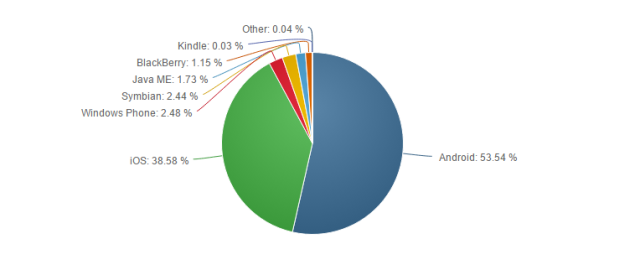
\includegraphics[width=17cm]{imgs/ch2_android_udzial_2.png}
    \caption
{Android – udział w rynku urządzeń mobilnych na świecie. (Źródło: portal android.com.pl, 09/2015)}
    \label{fig:android_udzial_zagranica}
\end{figure} 

\section{Rozwój systemu}
Niezwykle cenną informacją z punktu widzenia developerów, jest informacja o udziale poszczególnych wersji Android na urządzeniach posiadanych przez użytkowników. Dzięki niej mogą oni lepiej zoptymalizować swoje aplikacje pod kątem sprzętu. Dane z września 2015 przedstawiają się następująco:

\begin{figure}[!htb]
    \centering
    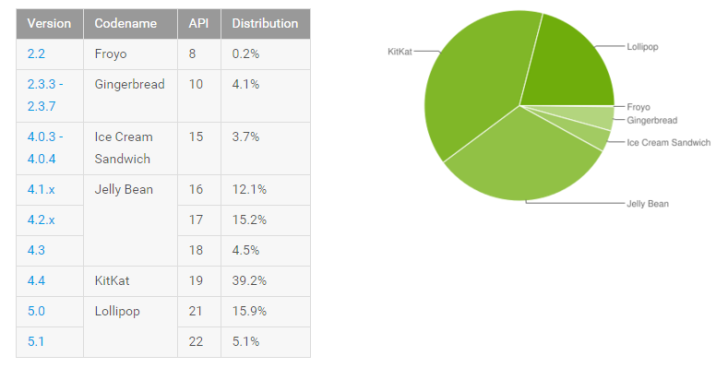
\includegraphics[width=17cm]{imgs/ch2_android_udzial_3.png}
    \caption
{Statystyki dotyczące używania poszczególnych wersji systemu Android przez użytkowników (Źródło: portal androidnow.pl, 09/2015). Ostatnio doszła wersja 6.0, ale jej udział na rynku urządzeń w obecnej chwili jest znikomy.}
    \label{fig:android_udzial_wersje}
\end{figure} 

Z urządzeń, na których instalowany jest Android, większość stanowią oczywiście smartfony i tablety. Ale nie tylko. Również urządzenia takie jak \textit{smart-watches}, \textit{smart-TVs}, akcesoria telewizyjne, konsole do gier, piekarniki, pralki, lodówki, satelity wysyłane w kosmos, a także najnowsze dziecko firmy Google - Google Glass, wspomagane są tym popularnym systemem operacyjnym. Co więcej, firmy motoryzacyjne zaczynają instalować Androida w swoich samochodach, rozbudowując w ten sposób platformę informacyjną i rozrywkową.

Zgodnie z manifestem założonej przez Google w 2007 roku grupy \textit{Open Handset Alliance} (OHA), Android został zbudowany z wykorzystaniem wielu różnych komponentów na licencji \textit{open source}. Zalicza się do nich przede wszystkim jądro Linux, niezliczone biblioteki programistyczne, kompletne interfejsy użytkownika, aplikacje i wiele wiele innych. Większość kodu systemu Android jest wydana na licencji \textit{Apache Software License} (ASL, v 2.0). Wyjątkiem jest jądro Linuxa, które wykorzystuje GPLv2 oraz projekt \textit{WebKit} korzystający z licencji BSD. 

Niestety nie wszystkie części kodu Androida są otwarte dla programistów. Nawet urządzenia z należącej do Google linii Nexus zawierają komercyjne sterowniki, kodeki, a nawet całe aplikacje. Jest to duże utrudnienie dla programistów pragnących poznać tajniki budowy tego systemu i próbujących wykorzystać je do tworzenia własnych aplikacji. Mimo wszystko, wielu developerów, nie pracując dla Google bezpośrednio, zaangażowanych jest w tworzenie kodu nowych wersji systemu Android. Nie jest to proste, bo z niezrozumiałych przyczyn firma utrzymuje większość informacji dotyczących rozwoju swojego flagowego produktu w tajemnicy.

W rozwijanie systemu są zaangażowani jednak nie tylko programiści. Wokół Androida zrzeszeni są również producenci procesorów, kości pamięci, urządzeń, ekranów i wielu innych części skłądających się na gotowy produkt.

\section{Programowanie w systemie w Android}
Jako system operacyjny dostępny nieodpłatnie, Android zrzesza przy sobie również ogromną społeczność developerów piszących aplikacje, które poszerzają funkcjonalność urządzeń. W sierpniu 2014 roku w Google Play (wcześniej Android Market), dostępnych było ponad 1,3 miliona aplikacji, zarówno komercyjnych, jak i darmowych.

Najpopularniejszymi językami programowania, w których pisze się aplikacje na Androida, są Java i C++ ze środowiskiem Android NDK. O ile język Java wydawać się może najrozsądniejszym wyborem na pierwszy rzut oka, o tyle wielu programistów używa również środowiska NDK. Jest to zestaw narzędzi, który pozwala realizować części aplikacji za pomocą kodu macierzystego języków takich jak C i C ++. Zazwyczaj środowisko to wykorzystuje się w celu pisania programów, które intensywnie wykorzystują CPU, takich jak silniki gier, przetwarzania sygnału i symulacji fizyki. Jednak deweloperzy muszą wziąć pod uwagę również wady takiego rozwiązania, które mogą nie do końca zbilansować korzyści. Natywny kod Androida na ogół nie powoduje zauważalnej poprawy wydajności, ale za to zawsze znacznie zwiększa złożoność aplikacji, który to problem i tak już jest dużym wyzwaniem dla programistów Java, co autor postara się przybliżyć w kolejnych rozdziałach. Podsumowując, z NDK należy korzystać tylko wtedy, jeśli uznamy, że jest to niezbędne dla wytwarzanej aplikacji, a nie dlatego, że lepiej czujemy się programując w języku C/C++. Zanim zdecydujemy się na to rozwiązanie, najpierw należy sprawdzić, czy androidowe API zapewnia funkcjonalność, jakiej potrzebujemy.

Java i C czy C++ to jednak nie wszystkie języki, których możemy użyć przy programowaniu aplikacji na Androida. Podczas szukania materiałów do tej pracy autor spotkał się z przykładami aplikacji napisanych w C\#, Delphi, czy nawet PHP. Stanowią one jednak tak mały udział, że nie będą one brane pod uwagę podczas analizy opisywanego problemu testowalności oprogramowania na ten system operacyjny.


%tutaj przykłady jak użyć poszczególnych konstrukcji
%Przykładowy rysunek \ref{fig:sample_figure}. Prztykładowa tabela %\ref{tab:sample_table}. Przykładowy odnośnik do bibliografi \cite{bib:kowalski_2015}. \textbf{Powodzenia!}


%\begin{figure}[!htb]
%    \centering
%    \includegraphics[width=10cm]{imgs/sample_figure.jpg}
%    \caption{Przykłady rysunek}
%    \label{fig:sample_figure}
%\end{figure} 

%\begin{table}[]
%\centering
%\caption{Przykładowa tabela}
%\label{tab:sample_table}
%\begin{tabular}{|l|l|}
%\hline
%\textbf{Nazwa} & \textbf{Wartość} \\ \hline
%Test           & 1.2              \\ \hline
%Kwiatek        & 5                \\ \hline
%\end{tabular}
%\end{table}